\section{NoSQL Support Architectural Overview}
\label{sec:designnosql}

Transparent access to different \ac{NoSQL} family databases and providers, e.g. Amazon DynamoDB, Google Cloud Storage, MongoDB, must be supported in the system. In this section we provide an architectural design to support the communication between the tenant and backend \ac{NoSQL} databases. We first discuss the integration mechanisms with the components implemented in \cite{Muhler2012} and \cite{gomez2012}, and then provide the required adaptations.

\subsection{Integration}

% the used protocol in gomez and muhler approach is soap over http
% in this one we need to marshal json over http
% aggregate dynamic routing functionalities
% because it is packed as a service unit, and service assembly, we must include in

 ServiceMix-mt is shipped with an \ac{HTTP} \ac{BC} which supports the \ac{SOAP} over \ac{HTTP} communication protocol. As discussed in Chapter \ref{chap:relatedworks}, most of the Cloud data store providers offer a REST interface for accessing, and modifying data. The payload format supported by most of the vendors, and specified in the CDMI specification is \ac{JSON} \cite{cdmispec2012}. Therefore, we find suitable the reuse of this component, and its enrichment with the required operations which are described in the following subsection. 
 
The packaging required to deploy the component as a \ac{SA} forces us to statically include the imported packages in the \ac{BC} \ac{SA}. Unlike in the \ac{SQL} architectural approach one, the deployed \ac{HTTP} endpoint configuration in this case references an endpoint which is addressed in the \ac{BC} the configuration refers to. Therefore, we can include the needed packages in the \ac{BC} and not in the \ac{SA}s containing the tenant-aware endpoint configurations.

\subsection{Architectural Overview}

The multi-tenant aware \ac{HTTP} \ac{BC} provides tenant isolation at the tenant level. As in the Servicemix-camel-mt, we extend the component and provide isolation at the tenant and user level.

The architectural design presented in Figure \ref{fig:designnosql} is similar to the one presented in \cite{gomez2012}. The main reason of this similitude is that we must extend the functionalities of the \ac{BC} rather than making a substantial architectural modification. 

\begin{figure}[htb]
	\centering
		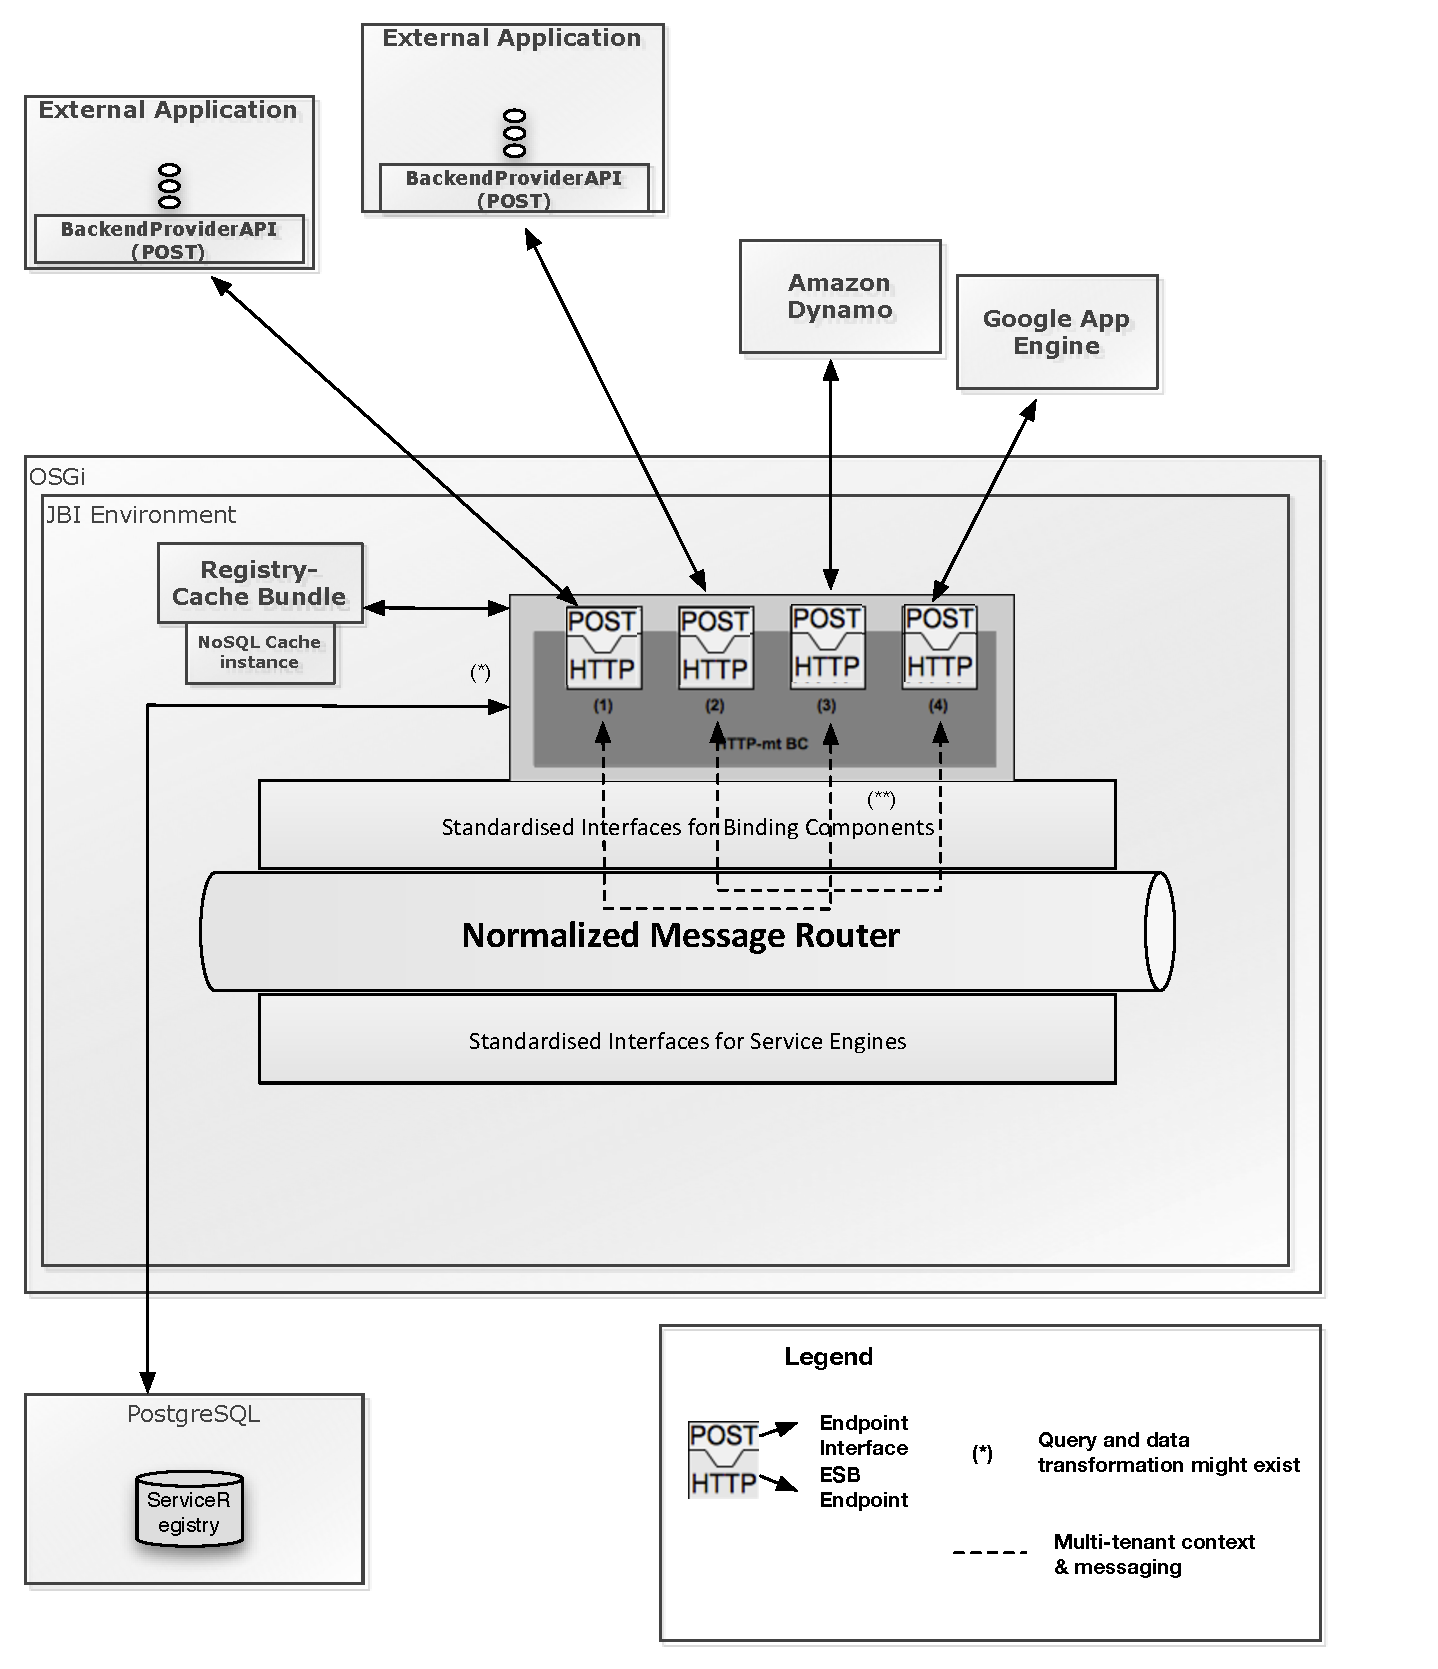
\includegraphics[clip, scale=0.5]{./gfx/nosqlApproach/noSqlApproachv3_doc.pdf}
	\caption[NoSQL Support]{Architectural overview of the design approach to support \ac{JSON} over \ac{HTTP} communication protocol and routing to \ac{NoSQL} data stores.}
	\label{fig:designnosql}
\end{figure}

In this approach we consider that the tenant in using the driver provided by the Cloud data store provider to access the consumer endpoint in ServiceMix-mt. The different Java SDKs which are offered by the providers support a set operations and data conversions, build the \ac{HTTP} request, and forward it to the data store endpoint. To support the different storage structures naming, authentication mechanisms, and data types, we extend the \ac{HTTP} \ac{BC} at the marshaling level, routing level, and enhance it with I/O operations with the service registry. Furthermore, to avoid adversely performance effects, it must support cashing mechanism. \ac{HTTP} provider endpoints are modified in order to able data retrieval from different backend data stores, as long as the source and target database's family and version are the same. 

When query or data transformation is needed, the message is forwarded from the \ac{HTTP} consumer to the transformer component's endpoint, which must then forward the message to the \ac{HTTP} provider endpoint.  

\FloatBarrier